\newpage
\section{Durchführung}\label{sec:durchfuehrung}
In diesem Kapitel werden die Szenarien im Detail beschrieben,
sowie deren Paketmittschnitte analysiert.
Die Analyse beschränkt sich hierbei auf Nachrichten der Pakete untereinander
und mit dem Szenario zusammenhängende Pakete an andere Geräte oder Server im Internet.


\subsection{Jeweils eine Minute ohne Aktionen bei ein- und ausgeschalteter Konsole}
Obwohl durch den Benutzer keine Aktionen angestoßen werden,
führen die Geräte verschiedene \enquote{Routineaufgaben} durch.

\paragraph{Home Assistant und Playstation 4}
Der Home Assistant wurde so konfiguriert,
dass er regelmäßig den Status der \ac{ps4} überprüft.
Dies geschieht über ein UDP-Paket,
welches an Port \texttt{987} der Broadcast-Adresse \texttt{255.255.255.255} gesendet wird.
Über das Sender an die Broadcast-Adresse wird erreicht,
dass der Router das Paket an alle lokalen Geräte verteilt.
Der Port wiederum ist der Port, über welchen die Playstation 4 UDP-Pakete annimmt.


Der Inhalt des Pakets (\autoref{lst:ps4-wakeup_search}) besteht aus dem Kommando \texttt{SRCH},
der HTTP-Version und einer \texttt{device-discovery-protocol-version}.
Vermutlich steht das Kürzel \texttt{SRCH} für \enquote{Search} und gibt damit an,
dass mit diesem Paket keine Aktionen ausgeführt,
sondern nur Systeminformationen mitgeteilt werden sollen.

\lstinputlisting[
    caption=Daten eines SRCH-Paketes,
    label=lst:ps4-wakeup_search
]{ps4_search.udp}

Auf dieses Paket Antwortet die \ac{ps4} ebenfalls mit einem UDP-Paket,
welches verschiedenen Geräteinformationen enthält.
Vergleicht man \autoref{lst:ps4-wakeup_search_respOn} und \autoref{lst:ps4-wakeup_search_respOff},
so ist festzustellen,
dass sich die jeweiligen Antworten lediglich im Statuscode der ersten Zeile unterscheiden.
\texttt{200 Ok} gibt an, dass die Playstation 4 eingeschaltet und \texttt{620 Server Standby},
dass die ausgeschaltet (bzw. im Standby) ist.

\lstinputlisting[
    caption=Antwort auf SRCH-Paket (Eingeschaltet),
    label=lst:ps4-wakeup_search_respOn
]{ps4_search_respOn.udp}

\lstinputlisting[
    caption=Antwort auf SRCH-Paket (Ausgeschaltet),
    label=lst:ps4-wakeup_search_respOff
]{ps4_search_respOff.udp}




\paragraph{Home Assistant und Harmony Hub}
Um ebenfalls regelmäßig den aktuellen Status der Spielekonsole zu erfahren,
erfrägt der Harmony Hub diese Information beim Home Assistant über die emulierte \textit{Hue Bridge}.
Dies geschieht in Form eines HTTP-GET-Requests,
welcher über eine für diesen Zweck errichte TCP-Verbindung erfolgt.
Der Request erfolgt and die URL \url{192.168.178.45:8300/api/12345678901234567890/lights}.
Über den Port \texttt{8300} wird die emulierte \textit{Hue Bridge} erreicht,
welche über den angegebenen Pfad Informationen über alle eingerichteten Leuchten bereitstellt.
Wie in Kapitel \ref{sec:aufbau-hassbian} \textit{\nameref{sec:aufbau-hassbian}} beschrieben zählt zu diesen Leuchten
auch der Schalter, über welchen sich die \ac{ps4} steuern lässt.

Als Antwort liefert Home Assistant mehrere Leuchten im JSON-Format.
Die Leuchte welche die Playstation 4 repräsentiert ist in \autoref{lst:ps4_get} dargestellt.
Hervorzuheben sind hier folgende Felder :
\lstinline[language=json]{"name"} enthält den nutzerfreundlichen Namen,
welcher in der Konfiguration angegeben wurde.
\lstinline[language=json]{"uniqueid"} enthält die
in der Konfiguration gesetzte ID mit dem zusätzlichen Präfix \lstinline[language=json]{"switch"}.
Das Feld \lstinline[language=json]{"on"} gibt an, ob die Leuchte (und damit die Spielekonsole) gerade eingeschaltet ist.
In diesem fall ist sie mit \lstinline[language=json]{false} ausgeschaltet.

\lstinputlisting[
    caption=Nutzdaten GET-Response (gekürzt),
    label=lst:ps4_get,
    language=json
]{ps4_get.json}


\subsection{Ein- und Ausschalten über \textit{Hassbian}}
\textit{Hassbian} bzw. der darin installierte Home Assistant bieten zur Steurung der konfigurierten Geräte eine Weboberfläche.
In \autoref{fig:hass-ui} ist der Schalter hervorgehoben, welcher für das Ein- und Ausschalten der Playstation 4 genutzt wird.

\begin{figure}[h!]
    \centering
    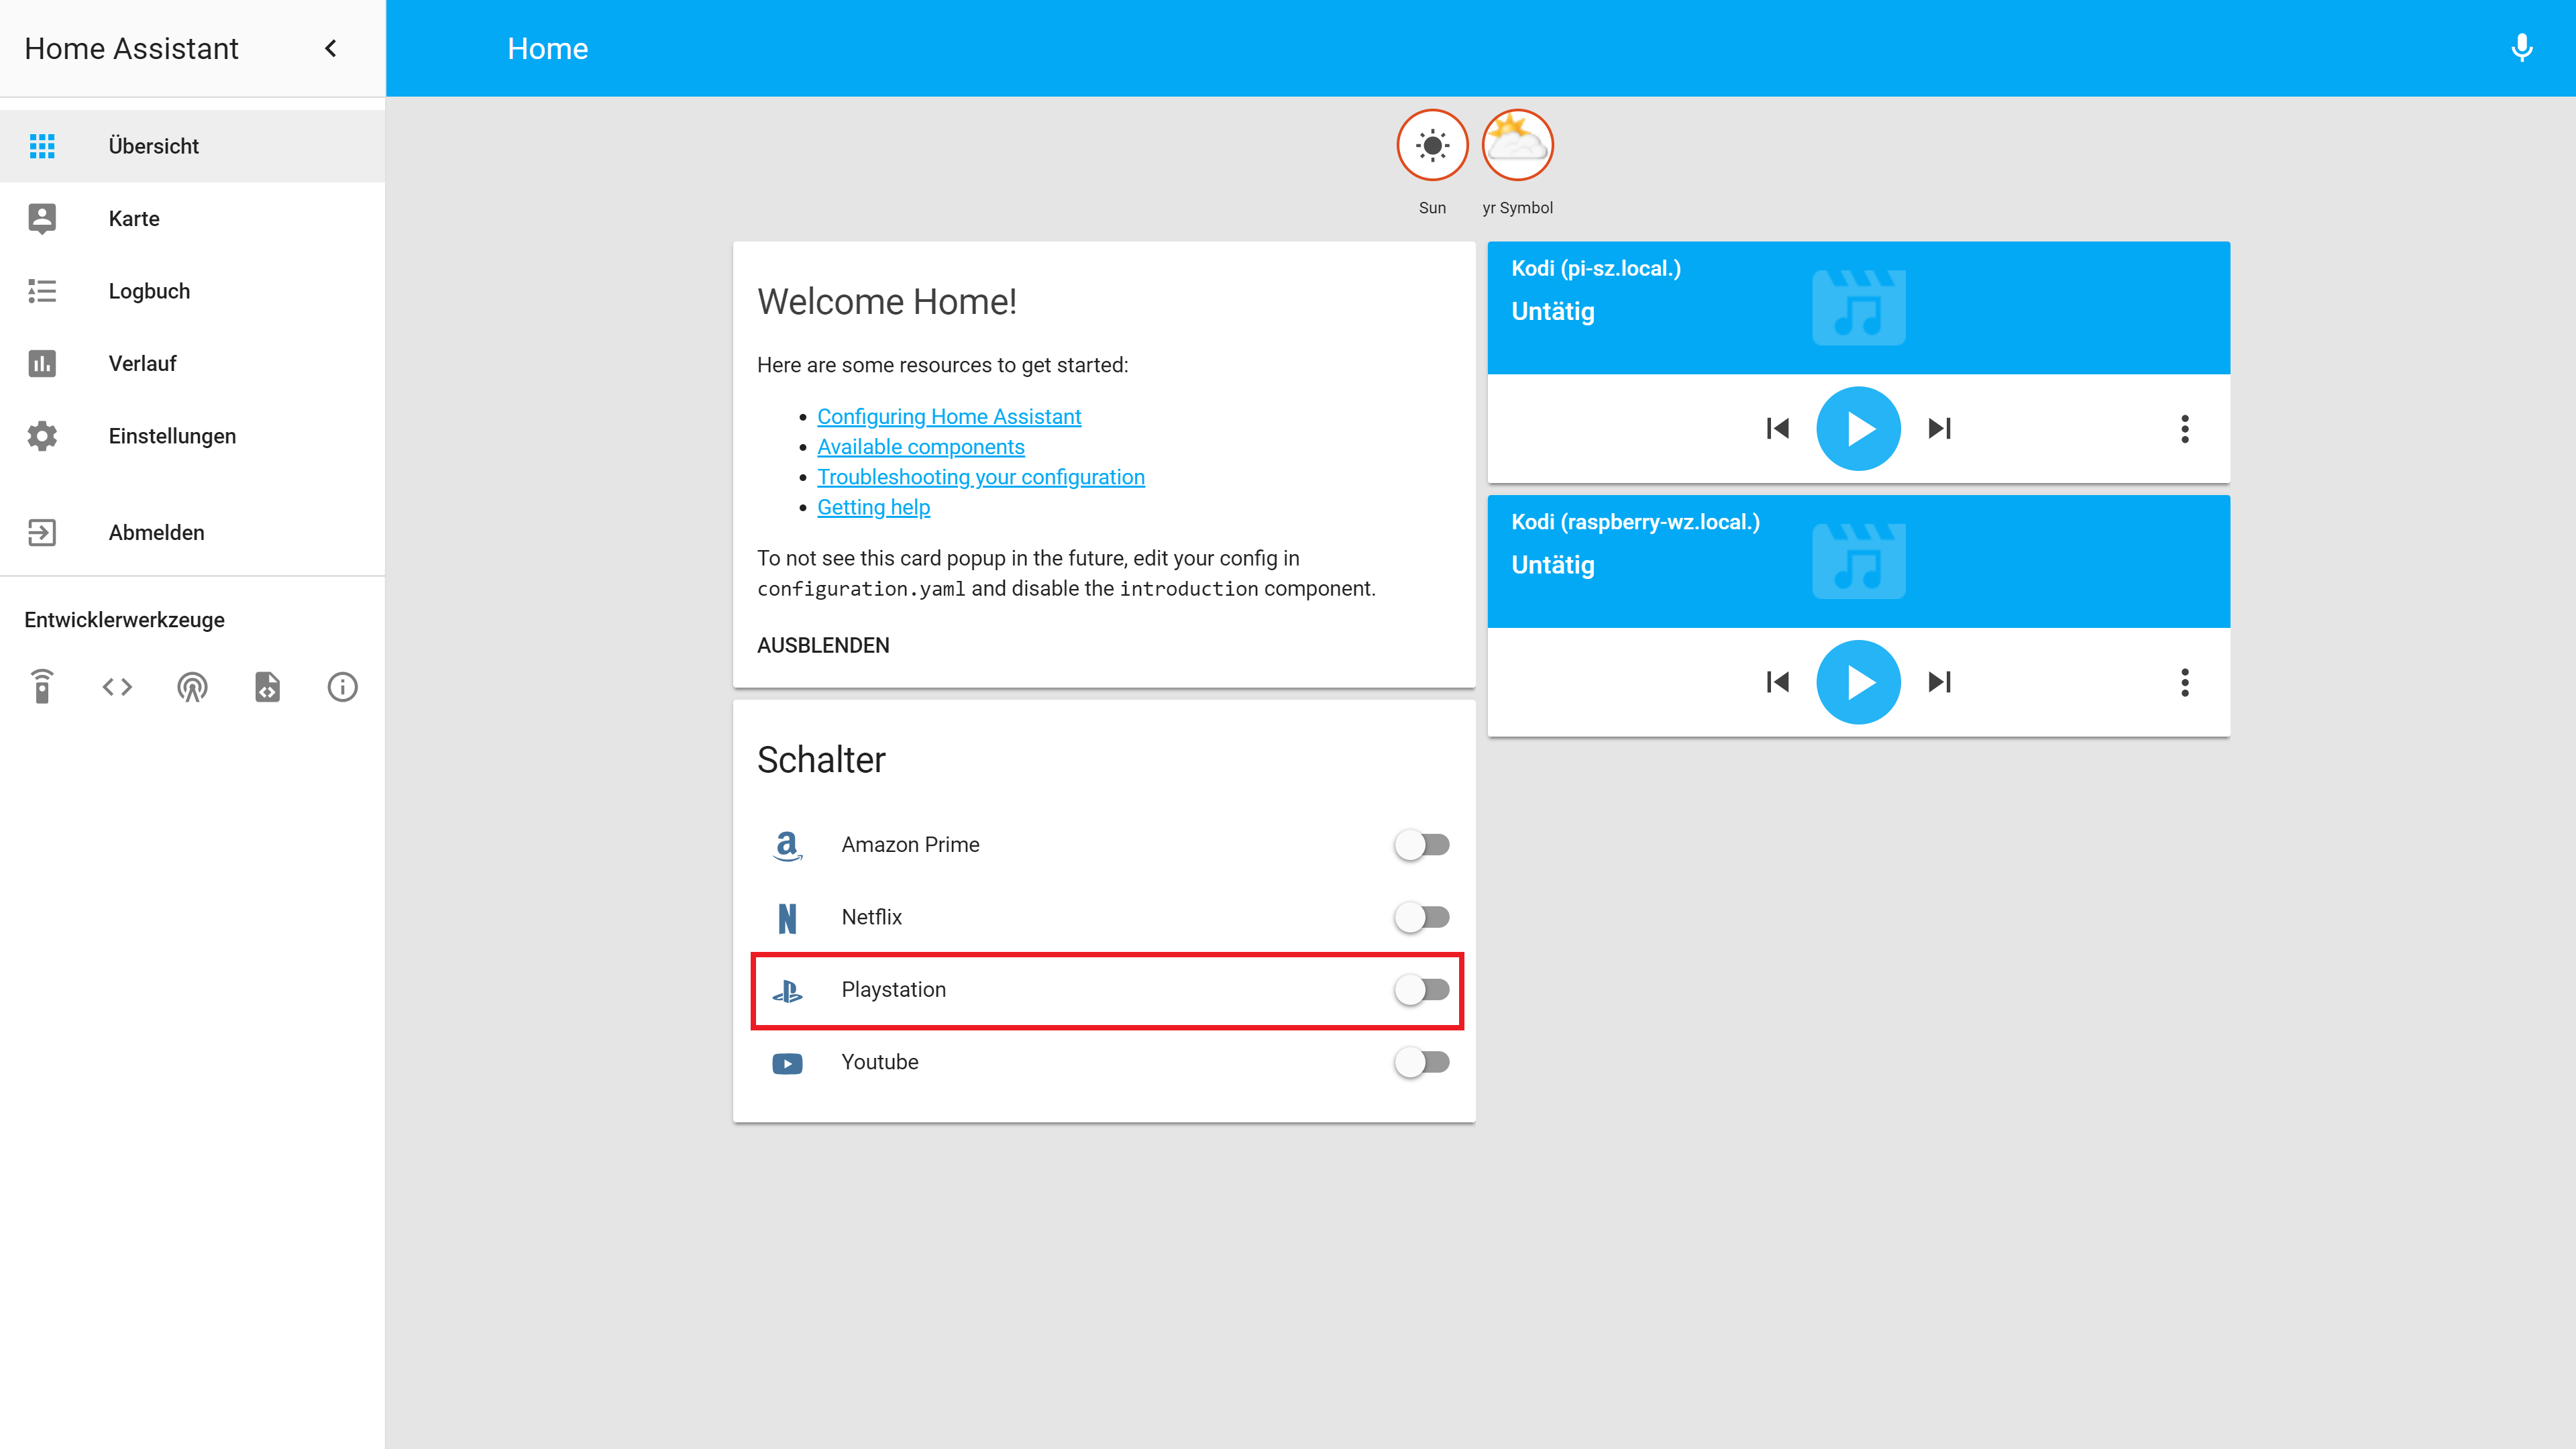
\includegraphics[width=\textwidth]{hass_ui}
    \caption{Weboberfläche des Home Assistant}\label{fig:hass-ui}
\end{figure}

\todo[inline]{Befehle auf Konfig verweisen}
Zum Einschalten wird der Befehl \texttt{ps4-waker -d 192.168.178.34 \\ -c \textasciitilde{}/.homeassistant/.ps4-wake.credentials.json} über das \ac{cli} abgesetzt.
Der Befehl weist das Programm \textit{ps4-waker} dazu an sich mit der Playstation 4 unter der IP-Adresse \texttt{192.168.178.34} zu verbinden und dabei die Zugangsdaten in der angegebenen JSON-Datei zu nutzen.

Das Ausschalten folgt nach einem ähnlichen Muster.
In dem Befehl wird noch das Kommando \texttt{standby} angehängt,
um die Playstation 4 auszuschalten (bzw. in den Ruhezustand zu versetzen). \\

Auch anhand der jeweiligen Paketmittschnitte ist ein gemeinsames Muster zu erkennen.
Der jeweilige Befehl wird mittels einer TCP-Verbindung Ausgeführt
während parallel mehrere UDP-Pakete in beide Richtungen gesendet werden.
Hierbei kommunizieren die beiden Geräte direkt miteinander.

Laut dem Entwickler dienen die UDP dazu, zu prüfen, ob die \ac{ps4} bereit ist eine Verbindung anzunehmen.
Hierzu werden zunächst zwei UDP-Pakete mit den in \autoref{lst:ps4-wakeup} gezeigten Daten
und dann ein UDP-Paket mit in \autoref{lst:ps4-launch} gezeigten Daten.
Das Feld \texttt{user-credential} (in den Listings gekürzt) ist hierbei immer gleich
und wurde beim Initialen Verbindungsaufbau ermittelt.

\lstinputlisting[
    caption=Daten eines WAKEUP-Paketes,
    label=lst:ps4-wakeup
]{ps4_wakeup.udp}

\lstinputlisting[
    caption=Daten eines LAUNCH-Paketes,
    label=lst:ps4-launch
]{ps4_launch.udp}

Der eigentliche Befehl wird dann in der auf die UDP-Pakete folgenden TCP-Verbindung ausgeführt.
Zwar ist diese Verbindung nicht mit TLS verschlüsselt, die Daten können dennoch nicht ausgelesen werden.
Die Ursache hierfür ist im Quellcode des \textit{ps4-waker} ersichtlich.
Die Daten werden dort vor dem Senden auf Anwendungsebene verschlüsselt.

\subsection{Ein- und Ausschalten über \textit{Harmony Hub} mittels Fernbedienung}
Im Harmony Hub ist zur Nutzung der Playstation 4 eine Aktion namens \enquote{Spielen} konfiguriert.
Zusätzlich zur Spielekonsole wird auch der Fernseher ein- bzw. ausgeschaltet sowie der entsprechende Eingangskanal gewählt.

Zum Einschalten wird der durch den Home Assistant bereitgestelle Schalter genutzt.
Über die emulierte \textit{Hue Bridge} erscheint dieser als Leuchte im Harmony Hub.

Ist die \ac{ps4} eingeschaltet, so kann der Hub eine Bluetooth-Verbindung aufbauen.
Daher ist es zum Ausschalten nicht nötig den Home Assistant zu nutzen.
Der Hub schlatet die Konsole direkt über die Bluetooth-Verbindung aus, sobald die Aktion beendet wird.

In dem Paketmittschnitt sind mehrere TCP-Verbindungen zu erkennen.
An der Kommunikation sind wie erwartet der Harmony Hub, \textit{Hassbian} und die \ac{ps4} beteiligt.
Zusätzlich frägt der Harmony Hub per DNS die IP-Adresse von \url{home.myharmony.com} an.
Als Antwort wird auf den Server an mit der URL \url{home-myharmony.us-east-1.elasticbeanstalk.com} verwiesen.
Interessant ist hierbei,
dass es sich hierbei um einen von Amazon gehosteten Server für Webanwendungen handelt \cite{AWSElast48:online}.

\textit{Hassbian} und die \ac{ps4} kommunizieren, wie bereits im vorigen Abschnitt untersucht, mittels TCP und UDP.
Der Harmony Hub kommuniziert mit \textit{Hassbian} über HTTP.

Der Ablauf der Kommunikation wird in \autoref{fig:ps-ein-harmony} vereinfacht dargestellt.
Bei HTTP-Verbindungen wird lediglich das HTTP-Paket gezeigt, der TCP-Rahmen mit Verbindungsauf- und abbau wird nicht abgebildet.

\begin{figure}[ht!]
    \centering
    \resizebox{\textwidth}{!}{
        \input{assets/uml/ps-ein-harmony.latex}
    }
    \caption{Übersicht Kommunikation beim Einschalten der \ac{ps4} über Harmony Hub}
    \label{fig:ps-ein-harmony}
\end{figure}

Der drei Verbindungen zum Server dienen vermutlich dazu Informationen über die gestartete Aktion mitzuteilen.
Dadurch wird ermöglicht, dass auch beispielsweise in der Smartphone-App ersichtlich ist, welche Aktion gerade aktiv ist.

Die Kommunikation zwischen \textit{Hassbian} und \ac{ps4} wurde bereits im vorigen Abschnitt betrachtet.
Der Paketmittschnitt zeigt, dass dies, wie zu erwarten, nach dem gleichen Schema abläuft.

Am Interessantesten ist in diesem Szenario die Kommunikation zwischen dem Harmony Hub und \textit{Hassbian}.
Diese findet über diverse HTTP-Requests (eingebettet in jeweils einer TCP-Verbindung) statt.
Diese Requests sprechen die emulierte \textit{Hue Bridge} über deren \ac{api} an.

\todo[inline]{Umschreiben dass nur noch put request}

Hierbei sind zwei unterschiedliche Requests zu erkennen:
\begin{description}
    \item[PUT]
        Der PUT-Request wird an die Adresse \url{http://192.168.178.45:8300/api/12345678901234567890/lights/1/state} gesendet.
        Der Server ist hier der \textit{Hassbian}, welcher an Port 8300 Befehle an die \textit{Hue Bridge} entgengennimmt.
        \texttt{/api/12345678901234567890/lights/1} wählt das zu kontrollierende Gerät aus.
        Wie in Kapitel \ref{sec:aufbau-hassbian} \textit{\nameref{sec:aufbau-hassbian}} beschrieben werden die Geräte nach außen hin als Lichter präsentiert.
        Als Nutzdaten enthält das Paket die \autoref{lst:ps4_on} gezeigten daten im JSON-Format.
        \lstinputlisting[
            caption=Nutzdaten PUT-Request,
            label=lst:ps4_on,
            language=json
        ]{ps4_on.json}
        Für diesen Anwendungsfall ist einzig der Wert \lstinline[language=json]{"on": true} von Relevanz.
        Mit dem Wert \lstinline[language=json]{"x,y"} könnte bei echten Lampen die Farbe
        und mit dem Wert \lstinline[language=json]{"bri"} die Helligkeit gesteuert werden \cite{Coreconc26:online}.
    \item[GET]
        Der GET-Request wird an die Adresse \url{http://192.168.178.45/api/12345678901234567890/lights} gesendet.
        Er dienst dazu Informationen zu den Geräten zu erfragen.
        Die Anfrage enthält keine weiteren Nutzdaten.
        Die Response hingehen entählt als Nutzdaten eine Auflistung aller verfügbaren Geräte mit deren Zustand.
        Eine gekürztes Beispiel ist in zu sehen.

\end{description}

Auffallend an den HTTP-Paketen ist,
dass sie ohne jegliche sicherheitstechnische Maßnahmen versendet werden.
Weder Integriät noch Vertraulichkeit sind gesichert.
Somit kann ein Angreifer, der sich im internen Netzwerk befindet,
sowohl die gesendeten Geräte passiv mitlesen und erfähr so,
welche Geräte im Netzwerk gesteuert werden.
Weitaus schlimmer ist jedoch, dass er die Anfragen auch selbst stellen kann.
Zum Einen muss er dann nicht (ggf. aufwändig) das Netzwerk belauschen
und zum Anderen kann er auf diesem Weg auch Geräte selbst steuern.

\todo[inline]{Ausschalten}

\subsection{Ein- und Ausschalten über \textit{Harmony Hub} mittels Smartphone-App}
Das Ein- bzw. Ausschalten der \ac{ps4} mittels der Smartphone-App fügt dem Szenario aus dem Vorkapitel eine weitere Abstraktionsebene Hinzu.
Anstatt direkt (über Funk) mit dem Hub zu kommunizieren,
wird die jeweilige Aktion über die Smartphone-App angestoßen.

